\newcommand{\insertForSmartphone}[1]{}

\newcommand{\compileForSmartphone}{
	\renewcommand{\insertForSmartphone}[1]{##1}
	\usepackage[a6paper,margin=5mm]{geometry}
}

\documentclass[a4paper,12pt,parskip=full]{scrreprt}

%\compileForSmartphone

\usepackage{acronym}
\usepackage{amsmath}
\usepackage{amssymb}
\usepackage{caption}
\usepackage{calc}
\usepackage[T1]{fontenc}
\usepackage{graphicx}
\usepackage{ifthen}
\usepackage[utf8]{inputenc}
%\usepackage[ngerman]{babel}
\usepackage{marvosym}
\usepackage{mathtools}
\usepackage{microtype}
\usepackage[colorlinks=false]{hyperref}
\usepackage{setspace}
\usepackage{subcaption}
\usepackage{tabu}
\usepackage{textcomp}
\usepackage[usenames,dvipsnames,svgnames,table]{xcolor}
\usepackage{tikz}

%\usepackage{csquotes}
%\usepackage[backend=biber,style=numeric-comp,sorting=none,maxnames=8,minnames=8,abbreviate=false]{biblatex} %sorting=nyt
%\addbibresource{literatur.bib}
%\DefineBibliographyStrings{ngerman}{
%	andothers ={{\textit{et\,al\adddot}}},
%}

\usetikzlibrary{arrows,decorations.pathreplacing}


\title{Slackforce: Documentation on the Theoretical Background}
%\subtitle{\thesisTitle}
\author{Tilman Sinning}


%\includeonly{abkuerzungsverzeichnis, einleitung,theorie,prozessierung,messverfahren,auswertung,ausblick,anhang}



\begin{document}

	\maketitle
	
	\tableofcontents

	% !TeX encoding = UTF-8
% !TeX spellcheck = en_US
% !TeX root = slackforceDocumentation.tex

\chapter{Introduction}

For slackliners it is often important to know the physical forces involved in slacklining, for example to estimate the suitability of potential slackline anchors. For static conditions, some well known calculations exist, to get the force on a slackline anchor from the sag of the slackline and the weight of the slackliner. However, it is often not easy to estimate the sag of a slackline precisely. Therefore it would be nice to have other measurement methods as well. Even more complicated is the estimation of the peak force in a slackline during dynamic movements like jumping.

The idea of the app ``Slackforce'' is to provide an easy to use solution for measuring and calculating forces in a slackline. This document describes the physical background and derivation of formulas and calculations used within this app. The app contains the following three main functionalities:

\begin{description}
	\item[Measure Force:] Measure the pretension of a slackline from the sound you hear when slapping the line with your finger.
	\item[Static Calculations:] Calculate the forces on a slackline at static conditions resulting from the geometric setup of the line.
	\item[Dynamic Simulation:] Simulate the movement and forces of a slackline during dynamic conditions like bouncing or jumping.
\end{description}

This document is divided into three chapters corresponding to the app functionalities. Note that the presented calculations are experimental and might contain errors. Use the formulas careful and do not fully trust the calculated values. The creator of this document is not responsible for any harm resulting from the use of the presented calculations and formulas.
	% !TeX encoding = UTF-8
% !TeX spellcheck = en_US
% !TeX root = slackforceDocumentation.tex

\chapter{Measure Force}

When slapping a tensioned slackline with your finger, you will hear a corresponding acoustical sound. The sound travels along the slackline as a mechanical wave and gets reflected at the end of the slackline. The propagation speed directly depends on the tension and the weight of the slackline. The idea is to calculate the pretension of the slackline from the time that sound needs to travel along the slackline back and forth. 

\section{Physical Background}

The propagation speed of a wave on a tensioned rope or slackline can be described with the following formula

\begin{equation}
v = \sqrt{\frac{F}{\mu_0}}
\label{eqn:speed1}
\end{equation}

where $v$ is the propagation speed, $F$ the force and $\mu_0$ the weight per unit length of the line. In between two sounds, the mechanical wave travels from one slackline anchor to the other and back, so it covers a distance two times the length $l$ of the line. If you measure the time of oscillation $t_{osc}$ the propagation speed can be calculated as:

\begin{equation}
	v = \frac{2\cdot l}{t_{osc}}
	\label{eqn:speed2}
\end{equation}

If you combine equation \ref{eqn:speed1} and \ref{eqn:speed2} and solve for the force you will get the following equation:

\begin{equation}
	F_0 = \frac{4\cdot l^2\cdot \mu_0}{t_{osc}^2}
	\label{eqn:measureForce}
\end{equation}

$F_0$ is the pretension of the line. As you can see, the weight and the length of the line have to be known. In the app the time of oscillation can be measured automatically with the microphone and some simple audio processing or manually by typing sound pattern on a button.

\section{The Influence of the Stretch Characteristic}

During the tensioning of the line, the line also stretches. As the total weight of the line does not change, this leads to a decrease of weight per unit length. Therefore equation \ref{eqn:measureForce} contains a systematic error on stretchy webbings. To take this into account a linear stretch behavior corresponding to the following formula is assumed.

\begin{equation}
	\frac{\Delta l}{l} = \alpha \cdot F
\end{equation}

where $\alpha$ is the stretch coefficient and $F$ is the force on the line. The corrected weight per unit length is calculated to

\begin{equation}
	\mu = \mu_0 \cdot \frac{1}{1+\alpha\cdot F}
\end{equation}

If you replace $\mu_0$ in formula \ref{eqn:measureForce} with the corrected value $\mu$ and solve the equation for F you get the following formula:

\begin{equation}
	F = \sqrt{\frac{1}{4 \alpha^2} + \frac{\mu_0\cdot 4l^2}{\alpha \cdot t_{osc}^2}} - \frac{1}{2\alpha}
	\label{eqn:measureForceWithStretch}
\end{equation}

In the App this more exact formula is used whenever a stretch coefficient greater than zero is entered.
It can be shown that formula \ref{eqn:measureForceWithStretch} equals formula \ref{eqn:measureForce} for $\alpha\rightarrow 0$.
	\chapter{Calculate Force}

The idea of calculating forces is to use the geometric information of the line and a known force to calculate unknown forces with simple vector algebra. If the tension of the line at a given sag is known the tension at a different sag can easily be calculated from the stretch behavior.

\section{Basics} \label{sec:basics}

\begin{figure}[htb] \centering
	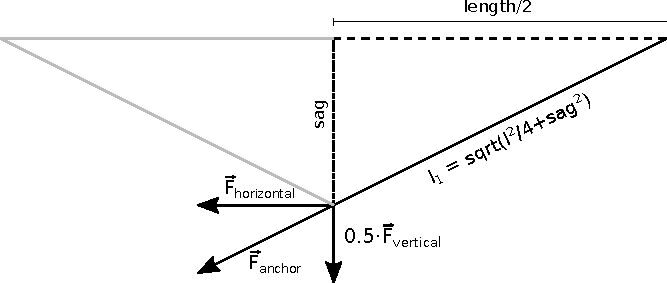
\includegraphics[width=0.8\textwidth]{images/slacklineWithForces.pdf}
	\caption{Schematical slackline with horizontal and vertical components of force}
	\label{fig:slacklineWithForces}
\end{figure}

Figure \ref{fig:slacklineWithForces} shows a schematical slackline with a given length and sag. As you can see it is possible to divide the force that affects the anchor of the line into a horizontal and a vertical component. The forces of the left part of the line will look the same. The total force will be the sum of forces on the left and the right side. So the horizontal components will eliminate each other and the vertical ones get added. If a slackliner is standing on the line the total vertical force has the amount corresponding to the slackliner's weight. From the geometric properties shown in figure \ref{fig:slacklineWithForces} the following equation can easily get extracted:


\begin{equation}
	\frac{F_a}{0.5\cdot F_v} = \frac{l_1}{s} = \frac{\sqrt{\frac{l^2}{4} + s^2}}{s^2}
\end{equation}

Together with the gravity acceleration $g = 9.81\frac{m}{s^2}$ and the weight of the slackliner $m$ this leads to the following four equations:

\begin{spreadlines}{1.5\baselineskip}
\begin{align}
	F &= \frac{\sqrt{s^2 + \frac{l^2}{4}}}{2\cdot s} \cdot m\cdot g \label{eqn:calcForce} \\
	m &= \frac{2\cdot s\cdot F}{g\cdot\sqrt{s^2 + \frac{l^2}{4}}} \label{eqn:calcWeight} \\
	s &= \sqrt{ \frac{m^2\cdot l^2\cdot g^2}{4\cdot(4F^2 - m^2g^2)} } \label{eqn:calSag} \\
	l &= \sqrt{ \frac{4\cdot s\cdot (4F^2 - m^2g^2)}{m^2g^2} } \label{eqn:calcLength} 
\end{align}
\end{spreadlines}

With Equation \ref{eqn:calcForce} - \ref{eqn:calcLength} it is possible to calculate any of the parameters force, weight of slackliner, sag and length if the other parameters are known.

\section{Calculating the Pretension}

\begin{figure}[htb] \centering
	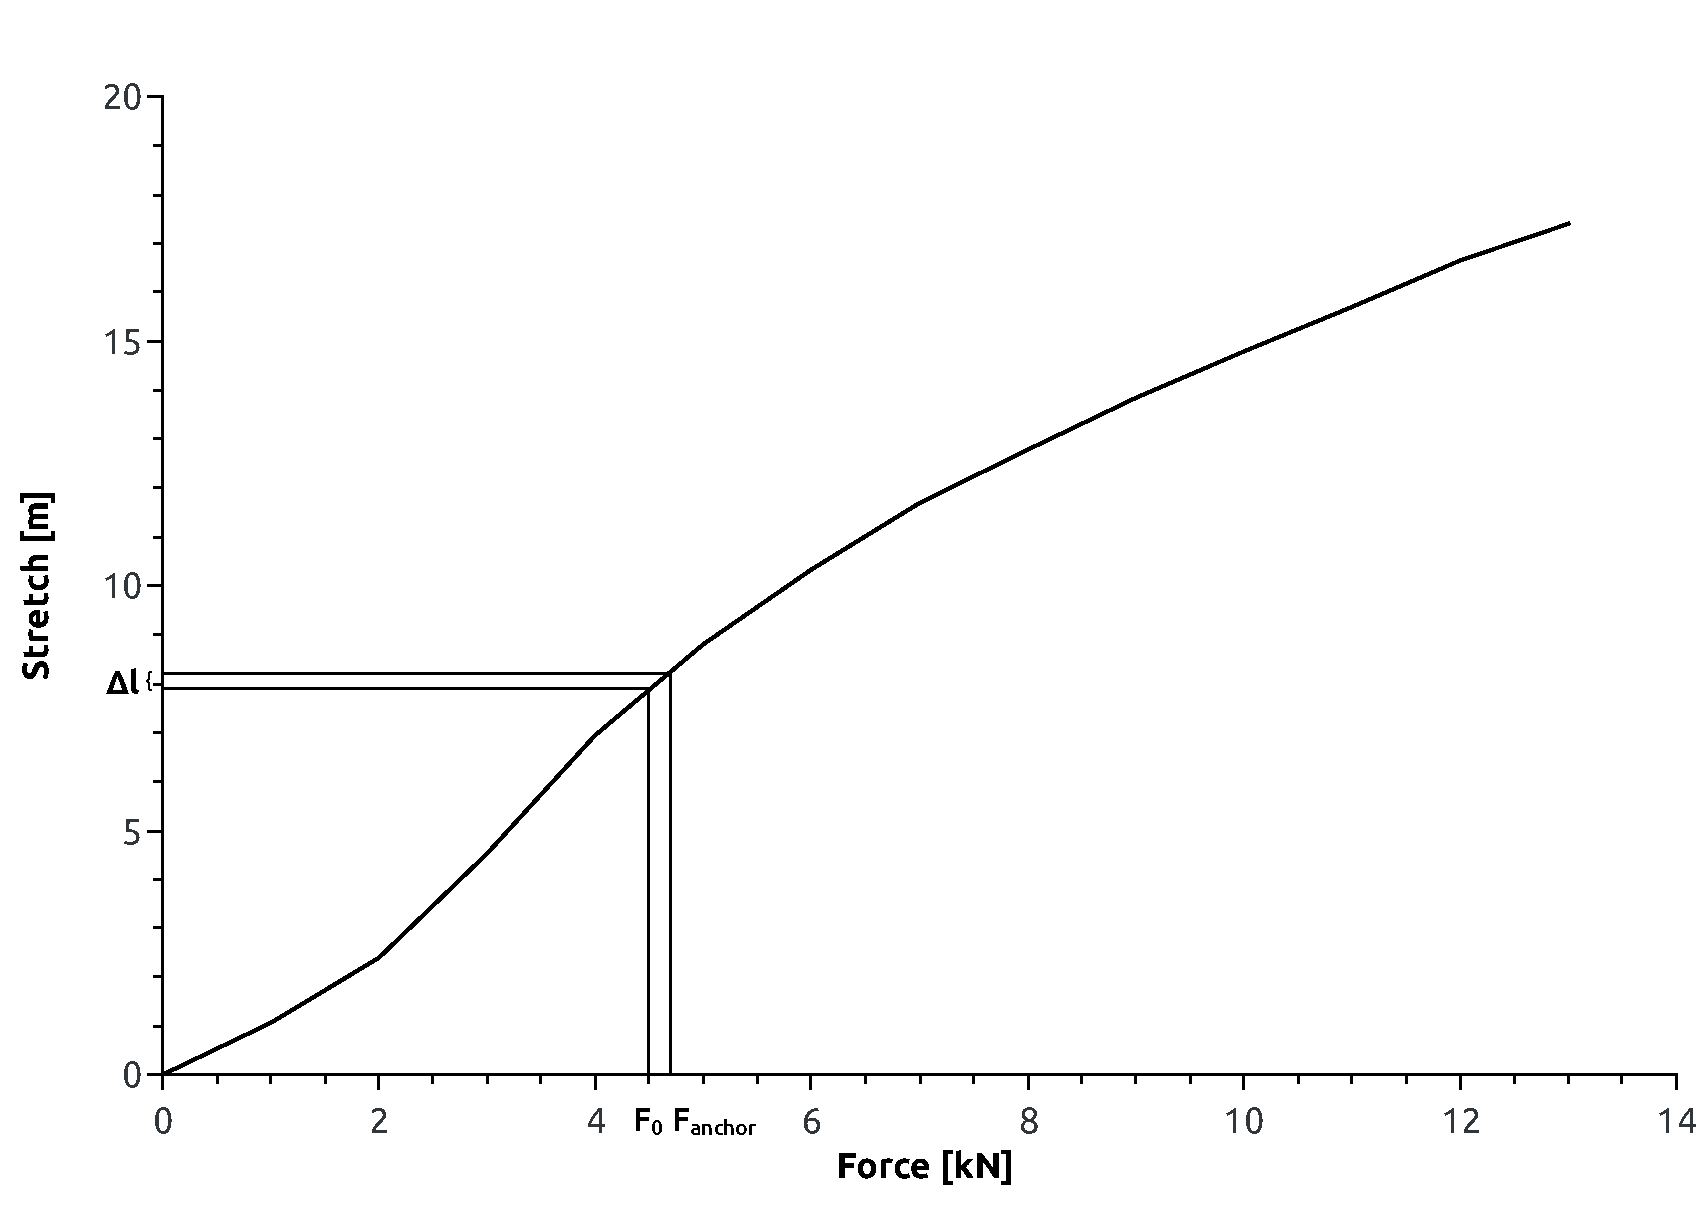
\includegraphics[width=0.8\textwidth]{images/forceStretchDiagram.pdf}
	\caption{Force-Stretch-Diagramm of a 100\,m Type 18 Line with 4,5\,kN Pretension}
	\label{fig:forceStretchDiagramm}
\end{figure}

If you know the tension with a person on a line and the stretch behavior it is possible to calculate the pretension. Figure \ref{fig:forceStretchDiagramm} shows the stretch behavior of a Type 18 MKII line as an example. Is can be seen that the stretch is not linear. To get the pretension of the line you need to know the increase of length $\Delta l$ due to the sag of the line. This can be calculated with the following formula:

\begin{equation}
	\Delta l = 2\cdot l_1 - l= 2\cdot \sqrt{s^2+\frac{l^2}{4}} - l
	\label{eqn:deltaL}
\end{equation}

To get the pretension you have to do the following steps:

\begin{enumerate}
	\item Calculate the anchor force with a slackliner on the line
	\item Read the corresponding stretch from the force-stretch-diagram
	\item Calculate the new stretch with formula \ref{eqn:deltaL}
	\item Read the pretension from the force-stretch-diagram
\end{enumerate}

If a linear stretch behavior $\frac{\Delta l}{l} = \alpha\cdot F$ is assumed it is possible to put that relation into an analytic formula:

\begin{equation}
	F = F_0 + \frac{2\cdot \sqrt{s^2+\frac{l^2}{4}} - l}{\alpha\cdot l}
\end{equation}

However, the App always uses the force-stretch-diagram as the results are better with that method. The diagram is interpolated linear between the provided data points. So the accuracy always depends on the number of available data points.

\section{Rodeo Lines}

Rodeo Lines are slacklines with a lot of sag and no pretension. So the pretension $F_0$ is always zero and the line has an initial sag $s_0$ without any slackliner on the line. When a slackliner steps on the line, it might stretch further and lead to a sag greater than the initial sag. Figure \ref{fig:RodeoLineWithForces} shows the forces on an rodeo line.

\begin{figure}[htb] \centering
	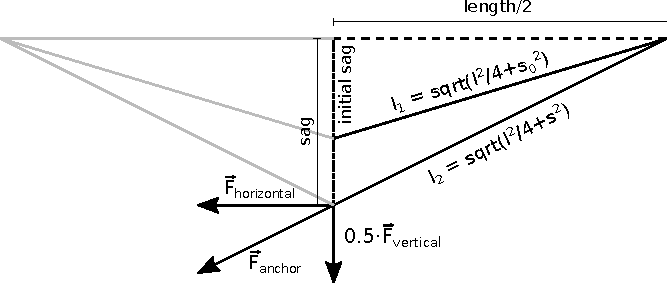
\includegraphics[width=0.8\textwidth]{images/rodeoLineWithForces.pdf}
	\caption{Schematical rodeo line with horizontal and vertical components of force}
	\label{fig:RodeoLineWithForces}
\end{figure}

As it can be seen there is no change to the static forces with a slackliner on the line from figure \ref{fig:slacklineWithForces}. So all the calculations of section ``\nameref{sec:basics}'' are still valid. If you want to do calculations based on the force-stretch-diagram you have to be aware that equation \ref{eqn:deltaL} now changes to

\begin{equation}
	\Delta l = 2\cdot (l_2 - l_1) = 2\cdot \left( \sqrt{s^2+\frac{l^2}{4}} - \sqrt{s_0^2+\frac{l^2}{4}}\right)
	\label{eqn:deltaLRodeo}
\end{equation}

In addition there is no pretension to calculate, but you can calculate the initial sag of the line using the force-stretch-diagram. Therefore you have to read the stretch $\Delta l$ from the diagram and use the following formula:

\begin{align}
	s_0 &= \sqrt{l_1^2 - \frac{l^2}{4}} = \sqrt{\left(l_2-\Delta l\right)^2 - \frac{l^2}{4}} \\
	&= \sqrt{\left( \sqrt{s^2 + \frac{l^2}{4}}  -\Delta l\right)^2 - \frac{l^2}{4}}
\end{align}

\section{Calculating Slackline Forces from the Pretension}

Unfortunately it is very difficult for linear stretch behavior and impossible for a custom stretch behavior to get an analytic expression of the slackline forces dependent on the pretension. Therefore some kind of approximation algorithm has to be used. The App is currently using the Illinois algorithm, that seems to work quite well.

\section{Slackliner not in the middle of the Line (not implemented)}

In the following it is assumed that the slackliner is standing at position $p \in [0,1]$ on the line. The forces always get calculated for the left anchor point. The forces at the right anchor point equal the forces at the left anchor point at position $1-p$. Figure \ref{fig:slacklineWithForcesUnsymmetric} shows the forces on this new setup. If the slackliner is not moving to the left or right the horizontal forces have to be the same on both sides. That leads to different vertical forces and anchor forces on both sides.

\begin{figure}[htb] \centering
	\begin{subfigure}{\textwidth} \centering
		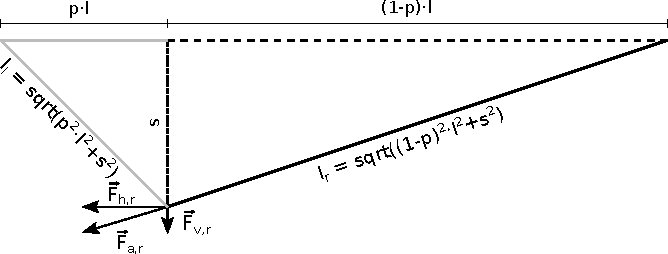
\includegraphics[width=0.8\textwidth]{images/slacklineWithForcesUnsymmetricRightSide.pdf}
	\end{subfigure} \par\bigskip
	\begin{subfigure}{\textwidth} \centering
		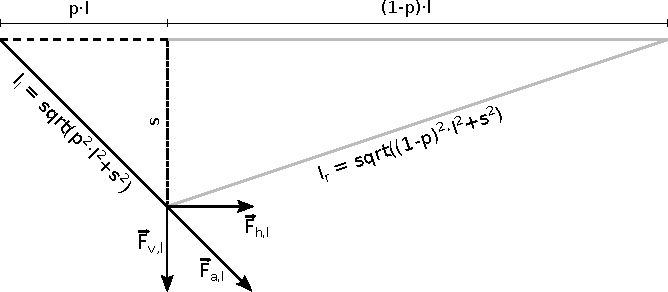
\includegraphics[width=0.8\textwidth]{images/slacklineWithForcesUnsymmetricLeftSide.pdf}
	\end{subfigure}
	\caption{Force Components on Unsymmetric Conditions }
	\label{fig:slacklineWithForcesUnsymmetric}
\end{figure}

From the geometrical properties follows

\begin{equation}
	\frac{p\cdot l}{s} = \frac{F_{h,l}}{F_{v,l}} = \frac{ \sqrt{F_{a,l}^2 - F_{v,l}^2 }}{F_{v,l}}
	\label{eqn:geometricPropertiesUnsymmetric}
\end{equation}

The the total vertical Force is still the sum of both sides:

\begin{equation}
	F_v = F_{v,l} + F_{v,r}
	\label{eqn:verticalForce}
\end{equation}

The equality of the horizontal forces leads to

\begin{equation}
	\frac{p\cdot l}{s}\cdot F_{v,l} = \frac{(1-p)\cdot l}{s}\cdot F_{v,r} 
	\label{eqn:horizontalEquality}
\end{equation}

The combination of equation \ref{eqn:horizontalEquality} and \ref{eqn:verticalForce} gives

\begin{equation}
	F_{v,l} = (1-p)\cdot F_v
	\label{eqn:leftVerticalForce}
\end{equation}

Inserting equation \ref{eqn:leftVerticalForce} in \ref{eqn:geometricPropertiesUnsymmetric} gives the final equation

\begin{equation}
	F_{a,l} = \frac{(1-p)\cdot F_v}{s}\cdot \sqrt{(p\cdot l)^2 + s^2}
\end{equation}

For $p = 0.5$ this equation is similar to equation \ref{eqn:calcForce} from the previous section. Note that equation \ref{eqn:deltaL} now changes to

\begin{equation}
	\Delta l = \sqrt{ (p\cdot l)^2 + s^2 } + \sqrt{ (1-p)^2 l^2 + s^2 } - l
\end{equation}







	\chapter{Dynamic Force Simulation}

In the previous section the calculations at static conditions were described. However, normally you do not just stand statically in the middle of a slackline. Often you want to do some bouncing or jumping which leads to a significant increase of force on the line. The goal of this section is to calculate those forces and get an idea of the influence of different setup parameters like length, pretension and stretch.

\section{Slackline as a Spring}

The simplest approach is to consider the slackline as a spring that can be described with the same formulas as in the previous section. Together with the following formulas and the formulas described in section \ref{sec:basics} it is easy to calculate the movement of the slackliner and the corresponding force:

\begin{align}
v(t) &= at+v_0 \\
s(t) &= \frac{a}{2}t^2 + v_0 t + s_0 \\
F &= a\cdot m
\end{align}

$a$ is the acceleration, $m$ the mass, $v$ the speed and $s$ the current sag. In a first version of the app the following iterative algorithm was used to simulate the movement of a slackliner: 

\begin{enumerate}
	\item Set the sag of the slackline to the current position of  the slackliner
	\item Calculate the force affecting the slackliner $F = m\cdot g - F_{v,slackline}$
	\item Calculate the acceleration of the slackliner $a = F / m$
	\item Calculate change in speed $\Delta v = a\cdot\Delta t$
	\item Calculate change in position $\Delta s = \frac{1}{2}\cdot a\cdot\Delta t^2 + v\cdot\Delta t$
	\item Calculate the current position and speed of the slackliner $s_{t+1} = s_{t} + \Delta s$, $v_{t+1} = v_{t} + \Delta v$
	\item Repeat steps 2 - 6
\end{enumerate}

However, this approach as some disadvantages. First from a numerical perspective it would be better to describe the movement of the slackliner with a differential equation and use a numerical approximation method for solving. But more important, dynamic measurements have shown that slacklines behave more like a viscoelastic material and not like a simple spring, that leads to a different behavior than shown above. To take this into account a more advanced model has to be used for the simulation.

\section{The Standard Linear Solid Model}

\begin{figure}[htb] \centering
	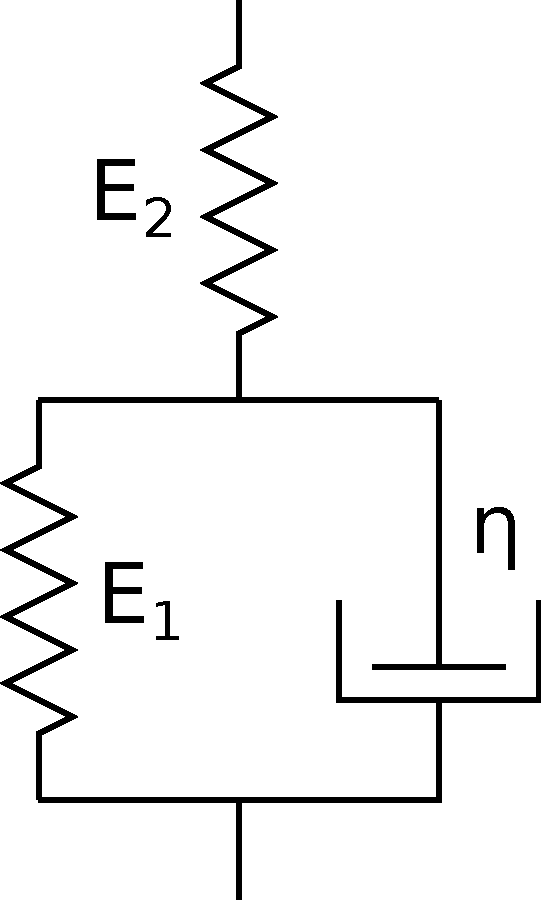
\includegraphics[width=0.4\textwidth]{images/dynamicStandardModel.pdf}
	\caption{Standard linear solid model}
	\label{fig:dynamicStandardModel}
\end{figure}

The standard linear solid model shown in figure \ref{fig:dynamicStandardModel} is a model to describe the behavior of viscoelastic materials. The springs and damper in the model can be described with the following equations:

\begin{align}
F_{k_1} &= k_1 \cdot x_1 \\
F_{k_2} &= k_1 \cdot x_2 \\
F_{d} &= d \cdot \dot x_2
\end{align}

From the connection of the elements in figure \ref{fig:dynamicStandardModel} follows:

\begin{equation}
	F_{k_1} = F_{k_2} + F_d
\end{equation}

Together with $x_1 + x_2 = x$ and $F = k_1 \cdot x_1$ the following equation can be derived:

\begin{equation}
	F + \frac{d}{k_1 + k_2} \dot F = \frac{k_1 \cdot k_2}{k_1 + k_2} x + \frac{d \cdot k_1}{k_1 + k_2} \dot x
	\label{eqn:linearSolidModel}
\end{equation}

With this equation the behavior of the slackline will be described in the following. For static conditions we have $\dot x_1 = 0$. Therefore the total spring constant $k_{ges} = \frac{k_1 \cdot k_2}{k_1 + k_2}$ can be described by the static stretch behavior of the slackline from the previous chapter with the following formula:

\begin{equation}
	k_{ges} = \frac{1}{\alpha \cdot l}
\end{equation}

So $k_1$ and $k_2$ are determined by the stretch coefficient which is known for many webbings and the ratio $\frac{k_1}{k_2}$ that might be similar on different webbings.

\section{Equation of Motion}

By looking at the equations from section \ref{sec:basics} again and considering that the acceleration of the slackliner has an additional input on the force in the dynamic case the force at the slackline anchor can be described with

\begin{equation}
	F = \frac{\sqrt{s^2 + \frac{l^2}{4}}}{2 \cdot s} \cdot F_{vertical} = \frac{\sqrt{s^2 + \frac{l^2}{4}}}{2 \cdot s} \cdot m\cdot (g - \ddot s)
\end{equation}

From the geometrics of the slackline the absolute stretch of one slackline half can be described with

\begin{equation}
	x = \frac{\Delta l_0}{2} + \sqrt{s^2 + \frac{l^2}{4}} - \sqrt{s_0^2 + \frac{l^2}{4}}
\end{equation}

where $\Delta l_0 = \alpha \cdot F_0 \cdot l$ is the initial stretch of the line due to pretensioning and $s_0$ is the initial sag of a rodeo line (either $\Delta l_0$ or $s_0$ is always zero). Derivating this equations with respect to the time results in the following two equations:

\begin{align}
	\dot F & \begin{multlined}[t]=  -\frac{l^2}{8}\cdot m \cdot (g - \ddot s) \frac{\dot s}{s^2 \cdot \sqrt{s^2 + \frac{l^2}{4}}} - \insertForSmartphone{\\}
	m \dddot s \frac{\sqrt{s^2 + \frac{l^2}{4}}}{2 \cdot s} \\
	\end{multlined}\\
	\dot x &= \frac{s \cdot \dot s}{\sqrt{s^2 + \frac{l^2}{4}}}
\end{align}

Inserting this equation into equation \ref{eqn:linearSolidModel} from the linear solid model and solving for $\dddot s$ leads to the following equation of motion:

\begin{equation}
\begin{split}
	\dddot s = \frac{k_1 + k_2}{d} \cdot (g - \ddot s) - 
	\frac{\dot s\cdot l^2}{4\cdot s \cdot l_2^2}\cdot (g - \ddot s) - \insertForSmartphone{\\}
	\frac{2sk_1k_2}{dml_2} \left(\frac{\Delta l_0}{2} + l_2 - l_1\right) - \frac{2s^2\dot s k_1}{ml_2^2}	
\end{split}
\label{eqn:equationOfEmotion}
\end{equation}

with

\begin{align}
	l_1 &= \sqrt{s_0^2 + \frac{l^2}{4}} \\
	l_2 &= \sqrt{s^2 + \frac{l^2}{4}}
\end{align}

As it can be seen we have a third order non linear differential equation now that can only be solved with numerical algorithms.

\section{Solving the Equation of Motion with the Runge-Kutta-Method }

To solve the equation of motion it has to be transformed into three first order differential equations:

\begin{align}
	\dot s &=G(s,v,a) = v \\
	\dot v &= H(s,v,a) = a \\
	\dot a &\begin{multlined}[t] = I(s,v,a) =\insertForSmartphone{\\} \frac{k_1 + k_2}{d} \cdot (g - a) - \frac{v\cdot l^2}{4\cdot s \cdot l_2^2} \cdot (g - a) - \\ \frac{2sk_1k_2}{dml_2} \left(\frac{\Delta l_0}{2} + l_2 - l_1\right) - \frac{2s^2v k_1}{ml_2^2} \\
	\end{multlined}
\end{align}

Now the equation can be solved iteratively with the Runge-Kutta-Method (4th order) with the following formula:

\begin{align}
	s_{t+1} &= s_t + \frac{1}{6} \cdot \Delta t \cdot (M_{1,i} + 2 M_{2,i} +2M_{3,i} +M_{4,i} ) \\ v_{t+1} &= v_t + \frac{1}{6} \cdot \Delta t \cdot (N_{1,i} + 2 N_{2,i} +2N_{3,i} +N_{4,i} ) \\
	a_{t+1} &= a_t + \frac{1}{6} \cdot \Delta t \cdot (O_{1,i} + 2 O_{2,i} +2O_{3,i} +O_{4,i} ) 
\end{align}

with 

\begin{align}
M_{1,i} &= G(s_i, v_i, a_i) \\
M_{2,i} &\begin{multlined}[t]= G \biggl(t_i + \frac{1}{2} \cdot \Delta t \cdot M_{1,i}, t_i + \frac{1}{2} \cdot \Delta t \cdot N_{1,i}, t_i + \insertForSmartphone{\\} \frac{1}{2} \cdot \Delta t \cdot O_{1,i}\biggr) \\\end{multlined} \\
M_{3,i} &\begin{multlined}[t]= G \biggl(t_i + \frac{1}{2} \cdot \Delta t \cdot M_{2,i}, t_i + \frac{1}{2} \cdot \Delta t \cdot N_{2,i}, t_i + \insertForSmartphone{\\} \frac{1}{2} \cdot \Delta t \cdot O_{2,i}\biggr) \\ \end{multlined} \\
M_{4,i} &\begin{multlined}[t]= G \bigl(t_i +  \Delta t \cdot M_{1,i}, t_i + \cdot \Delta t \cdot N_{1,i}, t_i + \insertForSmartphone{\\} \Delta t \cdot O_{1,i}\bigr)\\ \end{multlined}
\end{align}
\begin{align}
N_{1,i} &= H(s_i, v_i, a_i) \\
N_{2,i} &\begin{multlined}[t]= H \biggl(t_i + \frac{1}{2} \cdot \Delta t \cdot M_{1,i}, t_i + \frac{1}{2} \cdot \Delta t \cdot N_{1,i}, t_i + \insertForSmartphone{\\} \frac{1}{2} \cdot \Delta t \cdot O_{1,i}\biggr)\\ \end{multlined} \\
N_{3,i} &\begin{multlined}[t]= H \biggl(t_i + \frac{1}{2} \cdot \Delta t \cdot M_{2,i}, t_i + \frac{1}{2} \cdot \Delta t \cdot N_{2,i}, t_i + \insertForSmartphone{\\} \frac{1}{2} \cdot \Delta t \cdot O_{2,i}\biggr)\\ \end{multlined} \\
N_{4,i} &\begin{multlined}[t]= H \bigl(t_i + \Delta t \cdot M_{1,i}, t_i + \cdot \Delta t \cdot N_{1,i}, t_i + \insertForSmartphone{\\} \Delta t \cdot O_{1,i}\bigr)\\ \end{multlined}
\end{align}
\begin{align}
O_{1,i} &= I (s_i, v_i, a_i) \\
O_{2,i} &\begin{multlined}[t]= I \biggl(t_i + \frac{1}{2} \cdot \Delta t \cdot M_{1,i}, t_i + \frac{1}{2} \cdot \Delta t \cdot N_{1,i}, t_i + \insertForSmartphone{\\} \frac{1}{2} \cdot \Delta t \cdot O_{1,i}\biggr)\ \\ \end{multlined} \\
O_{3,i} &\begin{multlined}[t]= I \biggl(t_i + \frac{1}{2} \cdot \Delta t \cdot M_{2,i}, t_i + \frac{1}{2} \cdot \Delta t \cdot N_{2,i}, t_i + \insertForSmartphone{\\} \frac{1}{2} \cdot \Delta t \cdot O_{2,i}\biggr)\\ \end{multlined} \\
O_{4,i} &\begin{multlined}[t]= I \bigl(t_i +  \Delta t \cdot M_{1,i}, t_i + \cdot \Delta t \cdot N_{1,i}, t_i + \insertForSmartphone{\\} \Delta t \cdot O_{1,i}\bigr)\\ \end{multlined}
\end{align}


Unfortunately there are no measurements available characterizing the dynamic behavior of different webbings, so the parameters $\frac{k_1}{k_2}$ and $d$ can only be guessed. However, as a starting point there exists a document from \href{http://www.sigmadewe.com/fileadmin/user\_upload/pdf-Dateien/SEILPHYSIK.pdf}{Ulrich Leuthäusser} with some measurements on climbing ropes.
For the ropes tested there the ratio $\frac{k_1}{k_2}$ was always about $3$. The geometry independent damping factor $\delta = d \cdot l$ was varying between $\delta = 4.8 \dots 9\,kN\cdot s$.

	

\end{document}          
